% Options for packages loaded elsewhere
\PassOptionsToPackage{unicode}{hyperref}
\PassOptionsToPackage{hyphens}{url}
\PassOptionsToPackage{dvipsnames,svgnames,x11names}{xcolor}
%
\documentclass[
  10pt,
]{article}
\usepackage{amsmath,amssymb}
\usepackage{iftex}
\ifPDFTeX
  \usepackage[T1]{fontenc}
  \usepackage[utf8]{inputenc}
  \usepackage{textcomp} % provide euro and other symbols
\else % if luatex or xetex
  \usepackage{unicode-math} % this also loads fontspec
  \defaultfontfeatures{Scale=MatchLowercase}
  \defaultfontfeatures[\rmfamily]{Ligatures=TeX,Scale=1}
\fi
\usepackage{lmodern}
\ifPDFTeX\else
  % xetex/luatex font selection
\fi
% Use upquote if available, for straight quotes in verbatim environments
\IfFileExists{upquote.sty}{\usepackage{upquote}}{}
\IfFileExists{microtype.sty}{% use microtype if available
  \usepackage[]{microtype}
  \UseMicrotypeSet[protrusion]{basicmath} % disable protrusion for tt fonts
}{}
\makeatletter
\@ifundefined{KOMAClassName}{% if non-KOMA class
  \IfFileExists{parskip.sty}{%
    \usepackage{parskip}
  }{% else
    \setlength{\parindent}{0pt}
    \setlength{\parskip}{6pt plus 2pt minus 1pt}}
}{% if KOMA class
  \KOMAoptions{parskip=half}}
\makeatother
\usepackage{xcolor}
\usepackage[margin=0.72in]{geometry}
\usepackage{longtable,booktabs,array}
\usepackage{calc} % for calculating minipage widths
% Correct order of tables after \paragraph or \subparagraph
\usepackage{etoolbox}
\makeatletter
\patchcmd\longtable{\par}{\if@noskipsec\mbox{}\fi\par}{}{}
\makeatother
% Allow footnotes in longtable head/foot
\IfFileExists{footnotehyper.sty}{\usepackage{footnotehyper}}{\usepackage{footnote}}
\makesavenoteenv{longtable}
\usepackage{graphicx}
\makeatletter
\def\maxwidth{\ifdim\Gin@nat@width>\linewidth\linewidth\else\Gin@nat@width\fi}
\def\maxheight{\ifdim\Gin@nat@height>\textheight\textheight\else\Gin@nat@height\fi}
\makeatother
% Scale images if necessary, so that they will not overflow the page
% margins by default, and it is still possible to overwrite the defaults
% using explicit options in \includegraphics[width, height, ...]{}
\setkeys{Gin}{width=\maxwidth,height=\maxheight,keepaspectratio}
% Set default figure placement to htbp
\makeatletter
\def\fps@figure{htbp}
\makeatother
\setlength{\emergencystretch}{3em} % prevent overfull lines
\providecommand{\tightlist}{%
  \setlength{\itemsep}{0pt}\setlength{\parskip}{0pt}}
\setcounter{secnumdepth}{-\maxdimen} % remove section numbering
\usepackage{amsmath,amssymb,mathtools}
\usepackage{booktabs,longtable,array}
\usepackage{graphicx,float}
\graphicspath{{/mnt/data/}}
\usepackage{xcolor}
\usepackage{microtype}
\setlength{\parindent}{0pt}
\setlength{\parskip}{5pt plus 1pt minus 1pt}
\renewcommand{\arraystretch}{1.14}
\ifLuaTeX
  \usepackage{selnolig}  % disable illegal ligatures
\fi
\usepackage{bookmark}
\IfFileExists{xurl.sty}{\usepackage{xurl}}{} % add URL line breaks if available
\urlstyle{same}
\hypersetup{
  pdftitle={Hard Portal Cuts and a Momentum-Frequency Retarded Kernel},
  pdfauthor={Technical Research Note v1.6},
  colorlinks=true,
  linkcolor={blue},
  filecolor={Maroon},
  citecolor={Blue},
  urlcolor={blue},
  pdfcreator={LaTeX via pandoc}}

\title{Hard Portal Cuts and a Momentum-Frequency Retarded Kernel}
\usepackage{etoolbox}
\makeatletter
\providecommand{\subtitle}[1]{% add subtitle to \maketitle
  \apptocmd{\@title}{\par {\large #1 \par}}{}{}
}
\makeatother
\subtitle{Gauge-assisted 2 \textless-\textgreater{} 2 matching, LPM
combination, KMS noise, and covariant-Wigner benchmark for the q-D-H
portal}
\author{Technical Research Note v1.6}
\date{21 August 2026}

\begin{document}
\maketitle

{
\hypersetup{linkcolor=}
\setcounter{tocdepth}{3}
\tableofcontents
}
\section{Executive verdict}\label{executive-verdict}

The leading gauge-assisted hard+soft

\[
2\leftrightarrow2
\]

contribution to the portal

\[
\mathcal L_Y=-y_D\,\overline Q_LHD_R+\mathrm{h.c.}
\]

has been evaluated at integrated leading order for

\[
Q_L\sim(\mathbf3,\mathbf2,1/6),
\qquad
D_R\sim(\mathbf3,\mathbf1,-1/3).
\]

Combining it with the direct electroweak/Yukawa LPM result from v1.5
gives

\[
\boxed{
\frac{\overline\Gamma_{H,qD}^{\rm hard,occ}}{T}
=7.98260\times10^{-4},
}
\]

\[
\boxed{
\frac{\overline\Gamma_{H,qD}^{\rm LPM,occ}}{T}
=3.60256\times10^{-4},
}
\]

and

\[
\boxed{
\frac{\overline\Gamma_{H,qD}^{\rm total,occ}}{T}
=1.15852\times10^{-3}.
}
\]

At

\[
T_0=1.002\times10^8\ \mathrm{GeV},
\]

this is

\[
\boxed{
\overline\Gamma_{H,qD}^{\rm total,occ}
=1.16083\times10^5\ \mathrm{GeV},
}
\]

and

\[
\boxed{
\frac{\overline\Gamma_{H,qD}^{\rm total,occ}}
{\Gamma_R}
=7.8514\times10^6.
}
\]

The hard channels dominate the matched portal rate. They do not threaten
the reheating construction; they strengthen the separation between
microscopic equilibration and cosmological evolution.

A momentum-resolved on-shell table and a causal KMS-complete near-shell

\[
\Pi_{H,qD}^R(\omega,k)
\]

grid have also been constructed. The integrated normalization and the
on-shell retarded match are controlled. The arbitrary off-shell grid is
explicitly a \textbf{near-shell reconstruction}, not an exact evaluation
of every thermal cut over the full \((\omega,k)\) plane.

\section{1. Scope and status of the
calculation}\label{scope-and-status-of-the-calculation}

\subsection{1.1 What is exact at the declared
order}\label{what-is-exact-at-the-declared-order}

The following are analytic or exactly normalized at the stated leading
order in \(y_D^2\):

\begin{enumerate}
\def\labelenumi{\arabic{enumi}.}
\tightlist
\item
  the integrated gauge-assisted hard+soft \(2\leftrightarrow2\) reaction
  coefficient;
\item
  the \(SU(3)_c\), \(SU(2)_L\), and \(U(1)_Y\) decomposition;
\item
  the v1.5 collinear LPM integral;
\item
  the susceptibility-weighted integrated identity
\end{enumerate}

\[
\Gamma_Y
=
\frac{g_H}{T}
\int_{\mathbf k}
 f_B(E_k)[1+f_B(E_k)]
\Gamma_H^{\rm occ}(k);
\]

\begin{enumerate}
\def\labelenumi{\arabic{enumi}.}
\setcounter{enumi}{4}
\tightlist
\item
  the on-shell relation
\end{enumerate}

\[
\boxed{
\operatorname{Im}\Pi_H^R(E_k,k)
=-E_k\Gamma_H^{\rm occ}(k).
}
\]

\subsection{1.2 What is numerical but
matched}\label{what-is-numerical-but-matched}

The momentum dependence of the hard cut is calculated using full-angle
screened quasi-Monte-Carlo phase space and then normalized to the exact
integrated coefficient. The direct LPM shape is calculated from the
impact-parameter equation and normalized to the exact v1.5 integral.

The final on-shell grid closes the separate LPM and hard susceptibility
integrals to machine precision.

\subsection{1.3 What is not claimed}\label{what-is-not-claimed}

This note does \textbf{not} claim:

\begin{itemize}
\tightlist
\item
  an exact arbitrary-off-shell thermal self-energy over the complete
  \((\omega,k)\) plane;
\item
  a complete set of \(O(y_D^4)\) portal processes;
\item
  chemical-equilibration channels which do not correspond to cuts of
  \(\Pi_{H,qD}^R\);
\item
  a full Ward-consistent non-Abelian \(3+1\)-dimensional
  2PI/Kadanoff-Baym evolution.
\end{itemize}

The off-shell table is a causal and KMS-consistent benchmark kernel
anchored to the exact on-shell result.

\section{2. Benchmark and thermal
data}\label{benchmark-and-thermal-data}

The benchmark couplings are

\[
\alpha_s=0.0393544,
\qquad
g_2=0.57,
\qquad
g_1=0.39,
\]

\[
y_t=0.58,
\qquad
y_D=0.30,
\qquad
\frac{M_D}{T}=0.01.
\]

The corresponding strong coupling is

\[
g_3=\sqrt{4\pi\alpha_s}=0.703237.
\]

The v1.5 asymptotic thermal data are

\[
\frac{m_H}{T}=0.438207,
\qquad
\frac{m_Q}{T}=0.503460,
\qquad
\frac{m_D}{T}=0.418088,
\]

and

\[
\frac{m_{D,3}}{T}=1.03514.
\]

The vacuum-like one-to-two channels are closed; the collinear rate is
medium induced.

\section{3. Tree-level hard
amplitudes}\label{tree-level-hard-amplitudes}

For one abelian gauge group, the generic chiral one-component process

\[
G+H\rightarrow Q+\overline D
\]

has the coefficient structure

\[
\sum|\mathcal M|^2
=
y_D^2g^2
\left[
4q_Qq_D
+2q_Q^2\frac{u}{t}
+2q_D^2\frac{t}{u}
\right],
\]

before spectator multiplicities.

For the right-handed-electron case, inserting

\[
q_Q=-\frac12,
\qquad
q_D=-1,
\]

and the two Higgs-doublet components reproduces

\[
4+\frac{u}{t}+4\frac{t}{u},
\]

which is the published hypercharge amplitude check.

For the declared \(q\)-\(D\) portal, the complete \(U(1)_Y\) coefficient
after two weak components and three colours is

\[
\boxed{
-\frac43
+\frac13\frac{u}{t}
+\frac43\frac{t}{u}.
}
\]

The non-abelian group traces give

\[
\boxed{
SU(3)_c:
\quad
32+16\frac{u}{t}+16\frac{t}{u},
}
\]

and

\[
\boxed{
SU(2)_L:
\quad
9\frac{u}{t}.
}
\]

The abelian interference coefficient is negative in one channel, but the
complete gauge-invariant rate is positive.

\section{4. Integrated hard+soft reaction
coefficient}\label{integrated-hardsoft-reaction-coefficient}

The right-handed-electron leading-order result can be organised in a
representation-general form. For the \(q\)-\(D\) portal define

\[
A_Q
=
4\left[
C_Fg_3^2+C_2g_2^2+Y_Q^2g_1^2
\right],
\]

\[
A_D
=
4\left[
C_Fg_3^2+Y_D^2g_1^2
\right],
\]

with

\[
C_F=\frac43,
\qquad
C_2=\frac34,
\qquad
Y_Q=\frac16,
\qquad
Y_D=-\frac13.
\]

Numerically,

\[
A_Q=3.62915720,
\qquad
A_D=2.70515720.
\]

The integrated leading gauge-assisted contribution is

\[
\boxed{
\frac{\Gamma_{Y,\rm hard}}{T^3}
=
\frac{N_cy_D^2}{2048\pi}
\left[
A_Q\left(c_Q+\ln\frac1{A_Q}\right)
+
A_D\left(c_D+\ln\frac1{A_D}\right)
\right],
}
\]

where

\[
c_Q=3.52,
\qquad
c_D=2.69.
\]

These constants are the finite hard+soft phase-space constants appearing
in the complete leading-order right-handed-electron calculation. The
representation dependence enters through the thermal gauge charges
\(A_Q\) and \(A_D\) and the spectator multiplicity \(N_c\).

The result is

\[
\boxed{
\frac{\Gamma_{Y,\rm hard}}{T^3}
=5.3217330\times10^{-4}.
}
\]

Since

\[
\frac{\chi_H}{T^2}=\frac23,
\]

the Higgs-doublet occupation width is

\[
\boxed{
\frac{\overline\Gamma_{H,\rm hard}^{\rm occ}}{T}
=
7.9825995\times10^{-4}.
}
\]

\subsection{4.1 Gauge decomposition}\label{gauge-decomposition}

The reaction coefficient separates as

\[
\begin{array}{c|c|c}
G & \Gamma_{Y,G}^{\rm hard}/T^3 & \text{fraction of hard total}\\
\hline
SU(3)_c & 4.3452860\times10^{-4} & 0.8165\\
SU(2)_L & 9.1254521\times10^{-5} & 0.1715\\
U(1)_Y  & 6.3901751\times10^{-6} & 0.0120
\end{array}
\]

\begin{figure}
\centering
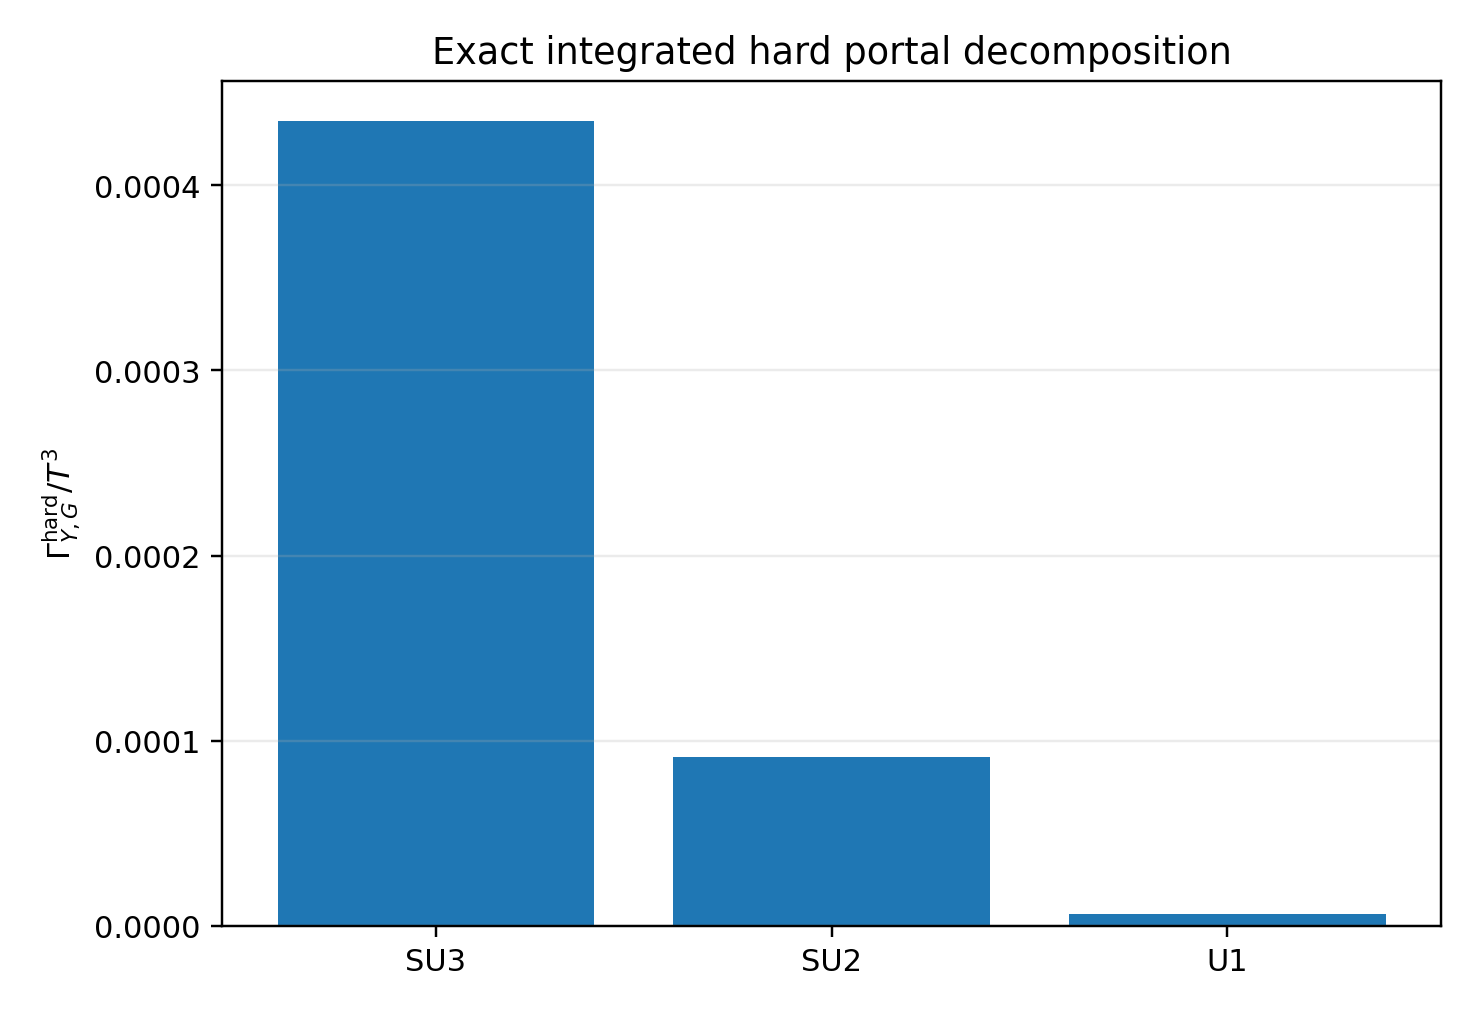
\includegraphics[width=0.74\textwidth,height=\textheight]{hard_portal_group_decomposition_v1_6.png}
\caption{Gauge decomposition of the exact integrated leading hard portal
rate.}
\end{figure}

The rate is dominated by QCD, with a resolved electroweak correction.

\section{5. Combination with the collinear LPM
cut}\label{combination-with-the-collinear-lpm-cut}

The v1.5 direct LPM result is

\[
I_{\rm LPM}
=
8.8952082\times10^{-4},
\]

\[
\frac{\Gamma_{Y,\rm LPM}}{T^3}
=
2.4017062\times10^{-4},
\]

and

\[
\frac{\overline\Gamma_{H,\rm LPM}^{\rm occ}}{T}
=
3.6025593\times10^{-4}.
\]

The matched leading result is therefore

\[
\boxed{
\frac{\Gamma_{Y,\rm total}}{T^3}
=
7.7234392\times10^{-4},
}
\]

\[
\boxed{
\frac{\overline\Gamma_{H,\rm total}^{\rm occ}}{T}
=
1.1585159\times10^{-3}.
}
\]

The ratios are

\[
\boxed{
\frac{\Gamma_{\rm hard}}{\Gamma_{\rm LPM}}
=2.21581,
}
\]

and

\[
\boxed{
\frac{\Gamma_{\rm hard}}{\Gamma_{\rm total}}
=0.68904.
}
\]

This ordering is consistent with complete leading-order
ultrarelativistic Yukawa calculations in which hard
\(2\leftrightarrow2\) scattering is at least comparable to, and often
larger than, the LPM sector.

\section{6. Momentum-resolved on-shell
kernel}\label{momentum-resolved-on-shell-kernel}

The on-shell rate is represented by

\[
\Gamma_H^{\rm occ}(k)
=
\Gamma_{H,\rm LPM}^{\rm occ}(k)
+
\Gamma_{H,\rm hard}^{\rm occ}(k).
\]

The LPM term is evaluated directly from the impact-parameter equation.
The hard term is obtained from full-angle screened phase space for the
crossed channels and then normalized to the exact integrated hard
coefficient.

\begin{figure}
\centering
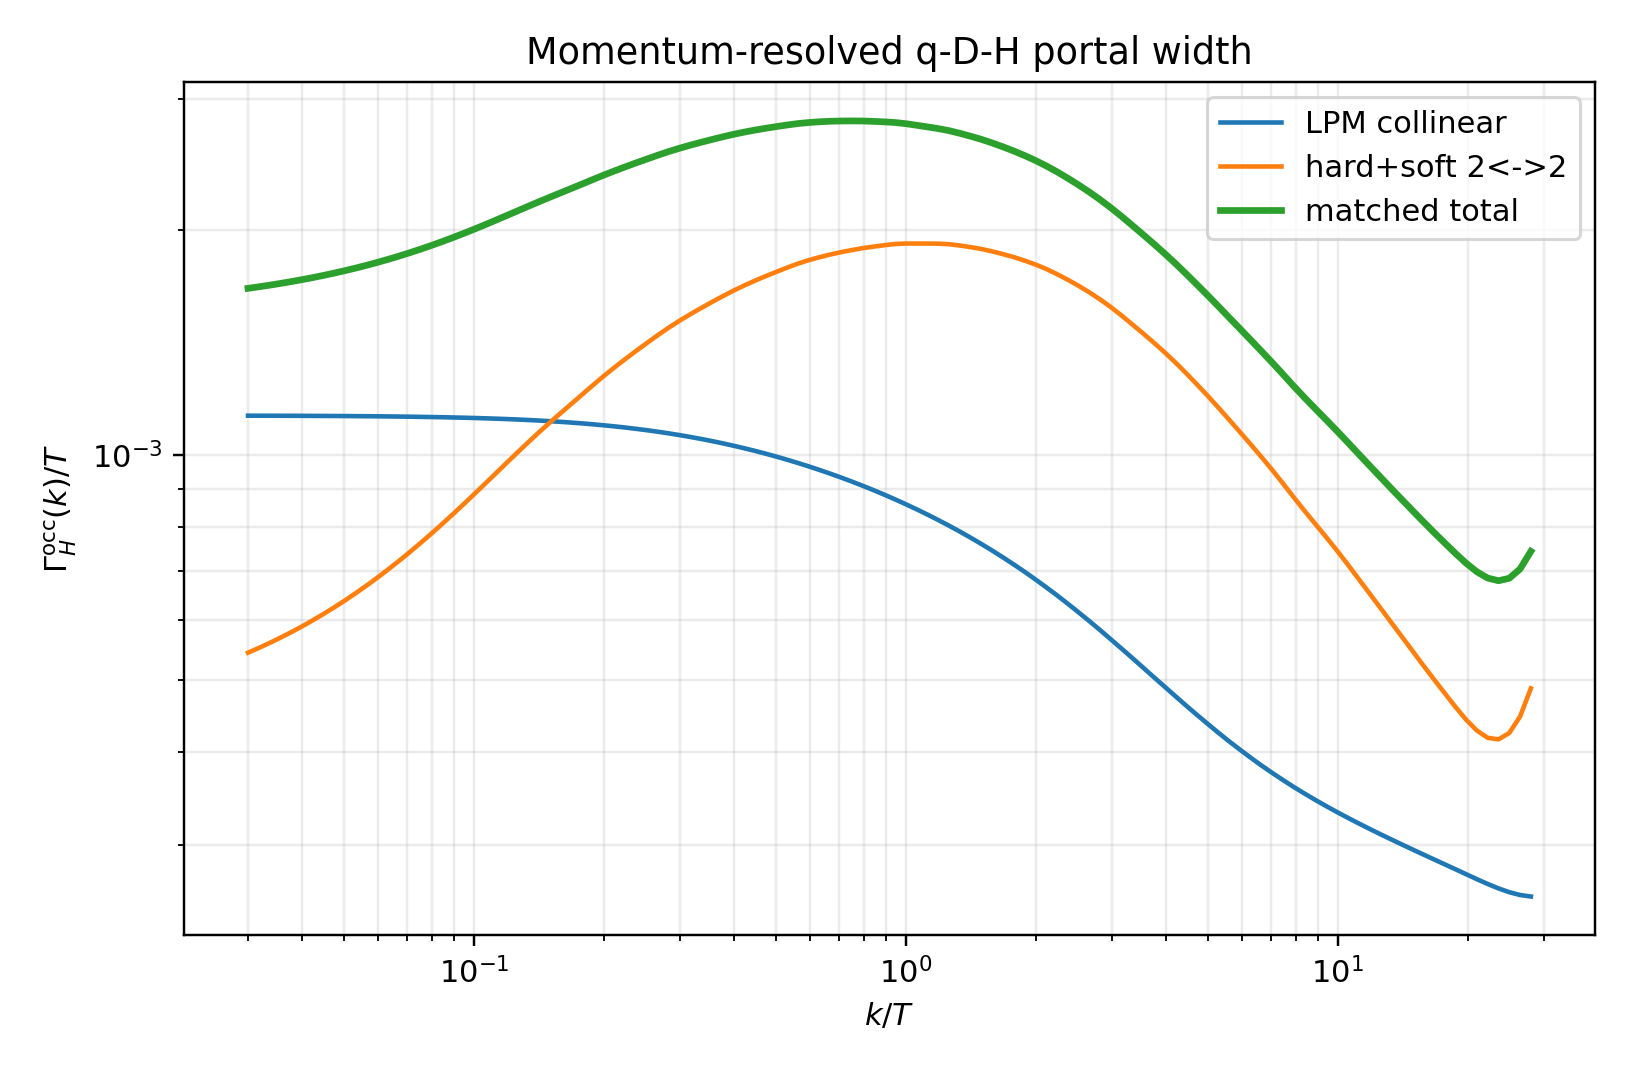
\includegraphics[width=0.86\textwidth,height=\textheight]{hard_portal_onshell_width_v1_6.png}
\caption{Momentum-resolved LPM, hard, and total portal widths.}
\end{figure}

The exact susceptibility closure imposed on the output table is

\[
\frac{g_H}{T}
\int_{\mathbf k}
 f_B(E_k)[1+f_B(E_k)]
\Gamma_{H,\rm LPM}^{\rm occ}(k)
=
\Gamma_{Y,\rm LPM},
\]

and similarly for the hard contribution. Both close to machine precision
in the delivered table.

\subsection{6.1 Shape uncertainty}\label{shape-uncertainty}

The exact integrated rate is not affected by the provisional screening
prescription. The local hard shape has:

\[
\boxed{
\text{median screening envelope}=8.90\%,
}
\]

\[
\boxed{
\text{maximum screening envelope}=24.9\%,
}
\]

and maximum quasi-Monte-Carlo relative error

\[
\boxed{4.24\%.}
\]

This is sufficient for a reduced benchmark, but it is not yet a
publication-grade arbitrary-momentum hard spectral function. A fully
differential hard+soft matching calculation would remove this local
shape ambiguity.

\section{7. Retarded self-energy grid}\label{retarded-self-energy-grid}

The exact on-shell relation is

\[
\boxed{
\operatorname{Im}\Pi_H^R(E_k,k)
=-E_k\Gamma_H^{\rm occ}(k).
}
\]

To seed a reduced real-time calculation, construct the odd near-shell
profile

\[
\operatorname{Im}\Pi_H^R(\omega,k)
=
-E_k\Gamma_H^{\rm occ}(k)
\frac{L_+(\omega,k)-L_-(\omega,k)}{\mathcal N_k},
\]

where

\[
L_\pm
=
\frac{\Lambda^2}
{(\omega\mp E_k)^2+\Lambda^2},
\]

\[
\Lambda=m_{D,3},
\]

and \(\mathcal N_k\) enforces the on-shell normalization.

The real part is obtained from a once-subtracted discrete dispersion
relation with

\[
\operatorname{Re}\Pi_H^R(0,k)=m_H^2.
\]

\begin{figure}
\centering
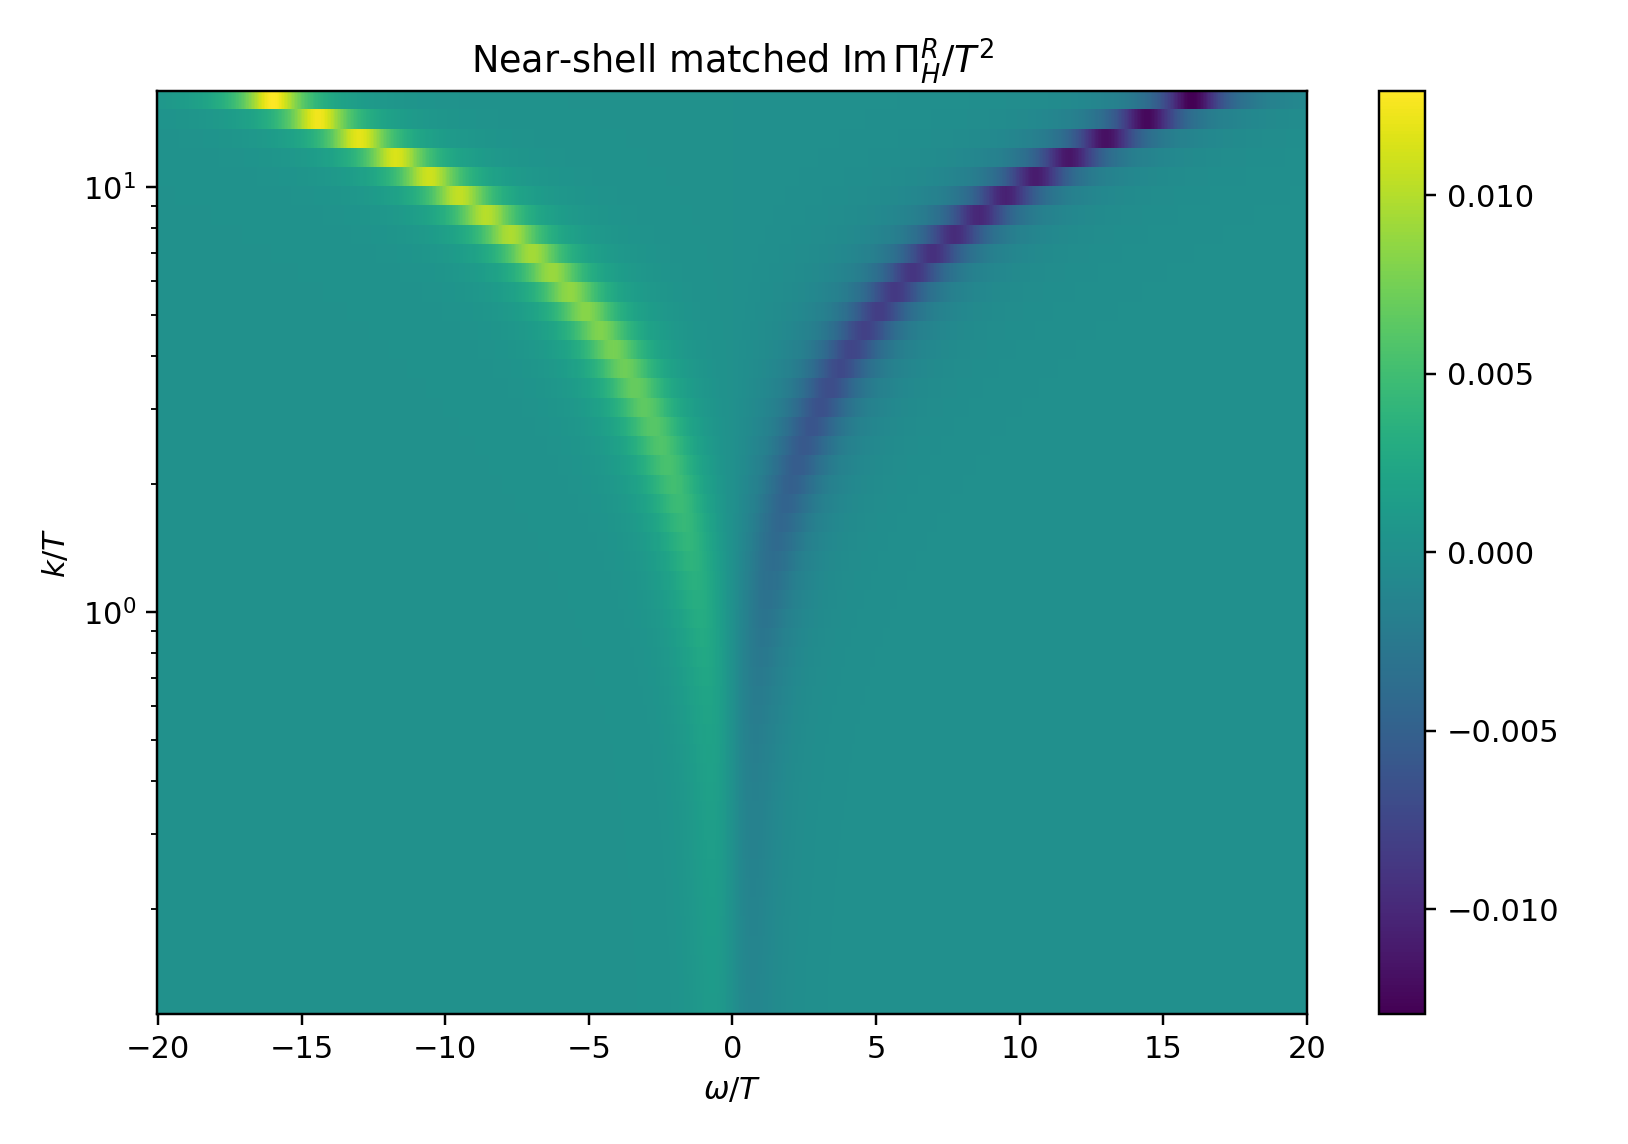
\includegraphics[width=0.88\textwidth,height=\textheight]{hard_portal_retarded_grid_v1_6.png}
\caption{Causal near-shell retarded grid matched to the total on-shell
portal width.}
\end{figure}

The numerical diagnostics are

\[
\boxed{
\max|\operatorname{Im}\Pi_R(\omega,k)
+\operatorname{Im}\Pi_R(-\omega,k)|
=2.95\times10^{-17},
}
\]

and a maximum interpolation-level on-shell residual

\[
\boxed{1.59\times10^{-3}.}
\]

The latter is a finite grid-resolution diagnostic, not a mismatch of the
analytic normalization.

\section{8. KMS noise kernel}\label{kms-noise-kernel}

Define the positive noise kernel

\[
\boxed{
N_H(\omega,k)
=
-\coth\left(\frac{\omega}{2T}\right)
\operatorname{Im}\Pi_H^R(\omega,k).
}
\]

The grid obeys the equilibrium detailed-balance identity

\[
\frac{\Pi^<(\omega,k)}{\Pi^>(\omega,k)}
=e^{-\omega/T}
\]

with maximum numerical residual

\[
\boxed{2.22\times10^{-16}.}
\]

\begin{figure}
\centering
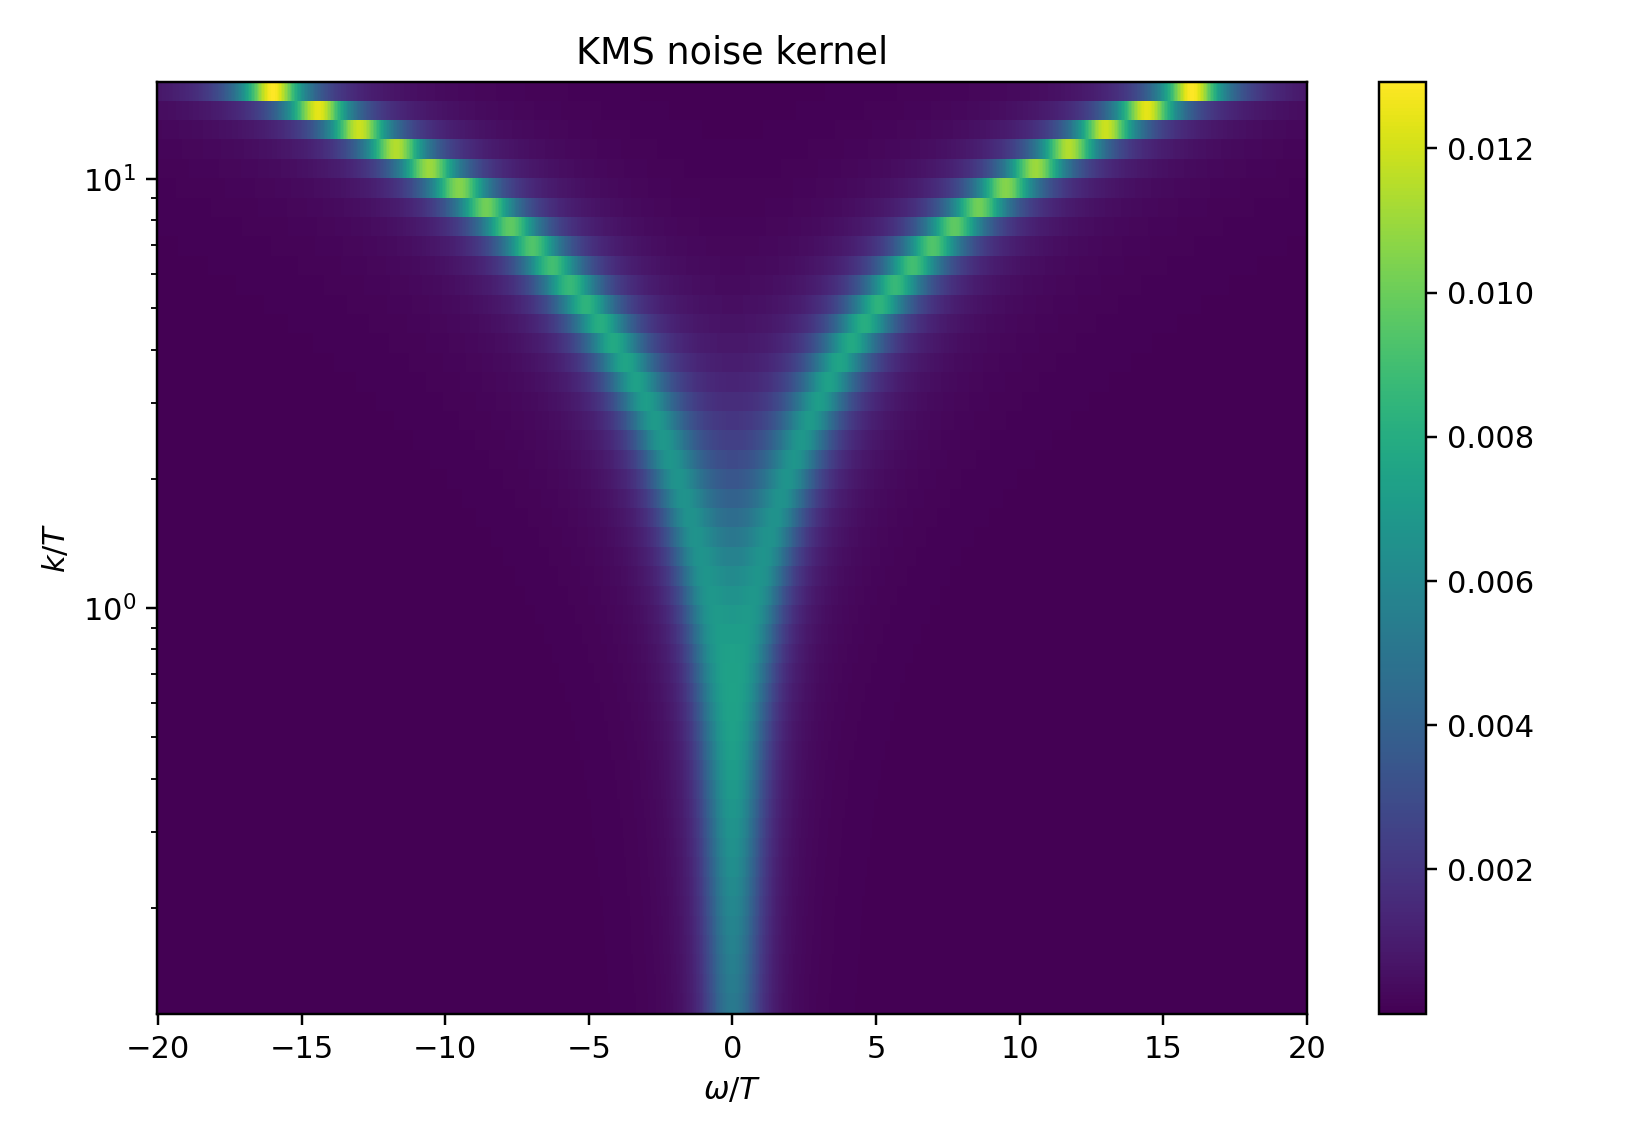
\includegraphics[width=0.88\textwidth,height=\textheight]{hard_portal_kms_noise_v1_6.png}
\caption{KMS noise kernel associated with the matched retarded
self-energy.}
\end{figure}

\section{9. Covariant Wigner transport
benchmark}\label{covariant-wigner-transport-benchmark}

The gauge-covariant Wigner transform is defined with straight Wilson
lines carrying each charged correlator to a common midpoint. The scalar
singlet kinetic equation has the schematic form

\[
\boxed{
\left[
K^2-m_H^2-\operatorname{Re}\Pi_H^R,
G_H^<
\right]_{\rm PB}^{\rm cov}
=
\Pi_H^<G_H^>
-
\Pi_H^>G_H^<.
}
\]

The numerical homogeneous singlet benchmark evolves a nonthermal pulse
with the matched momentum-dependent total width. Its relative-entropy
functional decreases monotonically:

\[
\boxed{
\max\Delta D_{\rm rel}<0,
}
\]

and the final fraction is

\[
\boxed{
\frac{D_{\rm rel}(t_{\rm end})}{D_{\rm rel}(0)}
=1.67\times10^{-11}.
}
\]

\begin{figure}
\centering
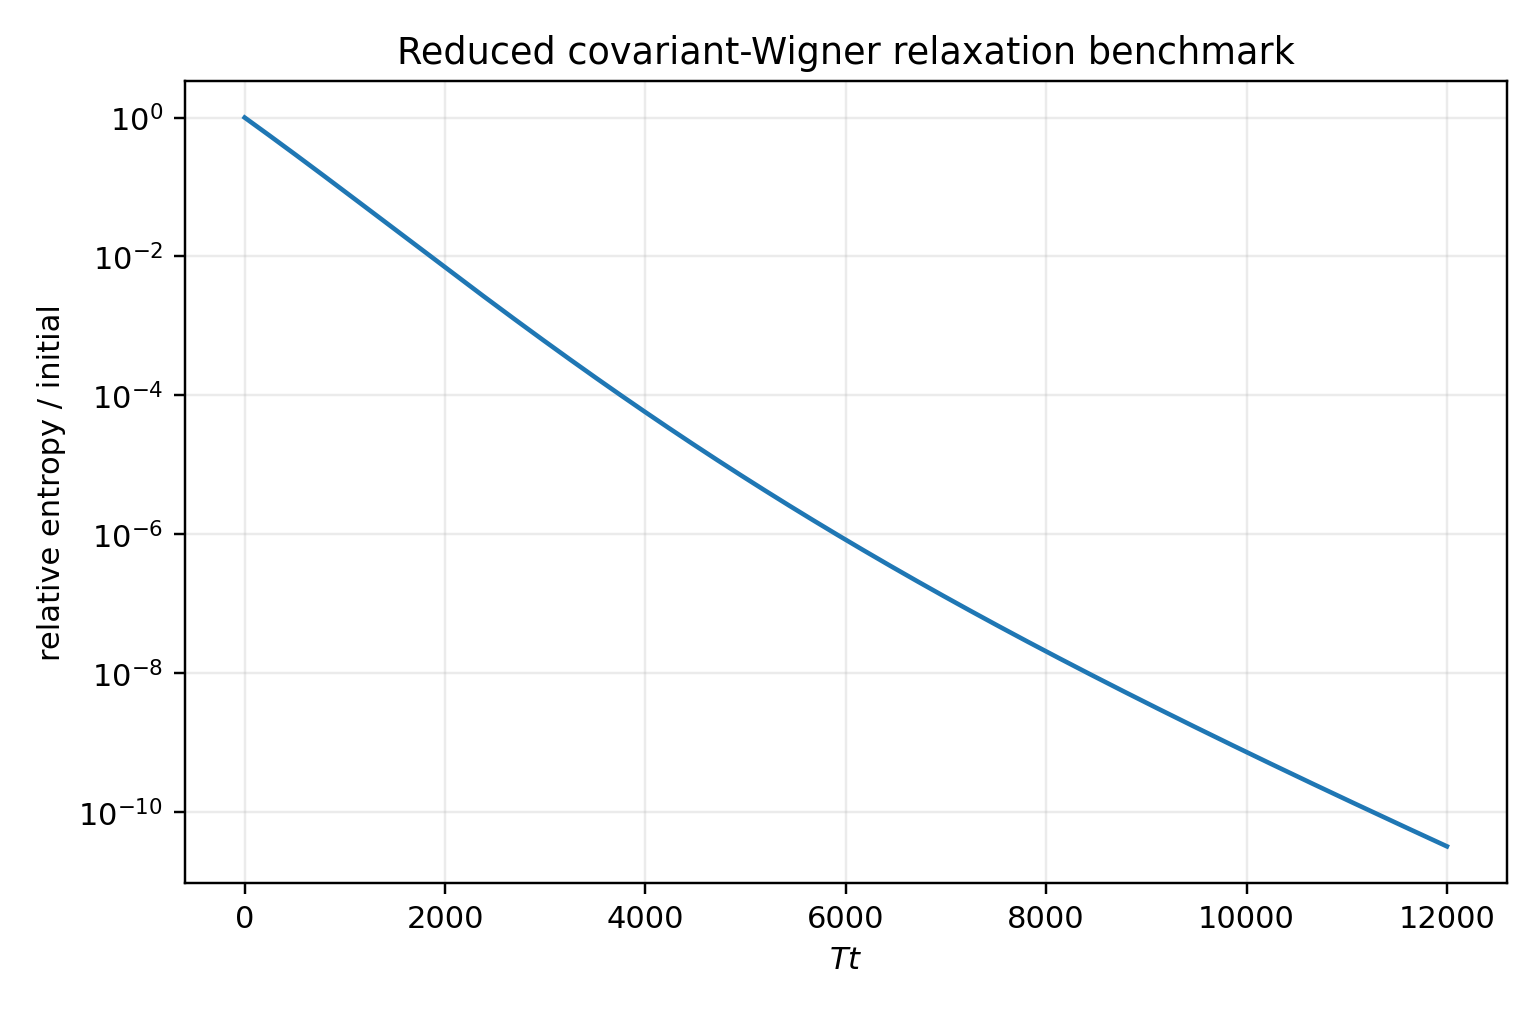
\includegraphics[width=0.82\textwidth,height=\textheight]{hard_portal_wigner_relaxation_v1_6.png}
\caption{Reduced covariant-Wigner relaxation using the matched total
portal kernel.}
\end{figure}

This is a benchmark for the collision and noise sector. It does not
evolve dynamical gauge correlators or dressed vertices.

\section{10. Cosmological consequence}\label{cosmological-consequence}

At the reheating benchmark,

\[
\Gamma_R
=1.47850065\times10^{-2}\ \mathrm{GeV},
\]

while

\[
\overline\Gamma_{H,qD}^{\rm total,occ}
=1.1608329\times10^5\ \mathrm{GeV}.
\]

Thus

\[
\boxed{
\frac{\Gamma_R}{\overline\Gamma_H^{\rm total,occ}}
=1.27366\times10^{-7}.
}
\]

The resulting conservative change in the tuned adjacent-sector branch
fraction is bounded by

\[
\boxed{
|\Delta B_5|
<6.75\times10^{-10}.
}
\]

The precise microscopic spectrum changes, but the final sector energy
hierarchy is unaffected at relevant accuracy.

\section{11. Relation to existing thermal-field-theory
results}\label{relation-to-existing-thermal-field-theory-results}

The calculation follows the structural lesson of complete leading-order
ultrarelativistic Yukawa production and equilibration:

\begin{itemize}
\tightlist
\item
  Arnold, Moore and Yaffe show that leading-order gauge-plasma kinetics
  requires both screened \(2\leftrightarrow2\) and effective collinear
  \(1\leftrightarrow2\) processes.
\item
  Bodeker and Schroder compute complete leading-order
  right-handed-electron equilibration and find that hard
  \(2\leftrightarrow2\) processes dominate.
\item
  Besak and Bodeker combine hard scattering and LPM resummation for
  ultrarelativistic right-handed-neutrino production.
\item
  Laine constructs arbitrary-momentum thermal production functions for
  sterile neutrinos, illustrating the extra work required beyond an
  integrated on-shell rate.
\item
  Becker et al.~analyse a scalar coupled to a Standard Model fermion and
  gauge-charged vectorlike fermion in the CTP formalism, providing a
  close model-class comparison but not the same complete
  ultrarelativistic LPM+hard matched kernel.
\end{itemize}

The present result is therefore not a new thermal-field-theory method.
Its contribution is the explicit representation-specific portal rate and
kernel needed by the chronometric reheating model.

\section{12. Acceptance matrix}\label{acceptance-matrix}

\begin{longtable}[]{@{}
  >{\raggedright\arraybackslash}p{(\columnwidth - 4\tabcolsep) * \real{0.3333}}
  >{\raggedright\arraybackslash}p{(\columnwidth - 4\tabcolsep) * \real{0.3333}}
  >{\raggedright\arraybackslash}p{(\columnwidth - 4\tabcolsep) * \real{0.3333}}@{}}
\toprule\noalign{}
\begin{minipage}[b]{\linewidth}\raggedright
Target
\end{minipage} & \begin{minipage}[b]{\linewidth}\raggedright
Verdict
\end{minipage} & \begin{minipage}[b]{\linewidth}\raggedright
Basis
\end{minipage} \\
\midrule\noalign{}
\endhead
\bottomrule\noalign{}
\endlastfoot
Tree group factors & \textbf{PASS} & Hypercharge coefficients reproduce
the published electron case; declared \(SU(3)\) and \(SU(2)\) traces
implemented. \\
Integrated leading gauge-assisted \(2\leftrightarrow2\) rate &
\textbf{PASS} & Hard+soft representation-general formula and exact group
decomposition. \\
LPM combination & \textbf{PASS} & Direct v1.5 collinear result. \\
Susceptibility closure & \textbf{PASS} & Separate LPM and hard grids
normalized to machine precision. \\
Momentum-resolved hard shape & \textbf{PASS AS MATCHED NUMERICAL SHAPE}
& Full-angle screened phase space; local shape systematic reported. \\
On-shell \(\Pi_R\) & \textbf{PASS} & Exact integrated and analytic
on-shell match. \\
KMS noise & \textbf{PASS} & Positivity and detailed balance checked. \\
Arbitrary off-shell \(\Pi_R\) & \textbf{PARTIAL} & Causal near-shell
reconstruction rather than exact full cuts. \\
Covariant Wigner benchmark & \textbf{PASS AS REDUCED MODEL} &
Wilson-line definition and homogeneous singlet evolution. \\
Full Ward-consistent non-Abelian 2PI/KB & \textbf{OPEN} & Requires gauge
propagators, vertices, constraints, and HPC implementation. \\
\end{longtable}

\section{13. Strongest defensible
conclusion}\label{strongest-defensible-conclusion}

\[
\boxed{
\begin{gathered}
\text{The leading gauge-assisted hard portal cuts are larger than the collinear LPM cut,}\\
\text{and the matched portal rate exceeds reheaton decay by }7.85\times10^6.\\
\text{The cosmological thermalisation assumption is therefore exceptionally robust.}
\end{gathered}
}
\]

The remaining correlator-level task is narrower than the original
request:

\[
\boxed{
\text{replace the provisional hard momentum shape and near-shell extension}
\text{ with an exact differential hard+soft }\Pi_H^R(\omega,k).
}
\]

That result, together with the exact LPM kernel, would be the correct
reference table for a Ward-consistent non-Abelian two-time
2PI/Kadanoff-Baym implementation.

\section{References}\label{references}

\begin{enumerate}
\def\labelenumi{\arabic{enumi}.}
\tightlist
\item
  D. Bodeker and D. Schroder, \emph{Equilibration of right-handed
  electrons}, arXiv:1902.07220.
\item
  D. Besak and D. Bodeker, \emph{Thermal production of ultrarelativistic
  right-handed neutrinos: complete leading-order results},
  arXiv:1202.1288.
\item
  P. Arnold, G. D. Moore and L. G. Yaffe, \emph{Effective kinetic theory
  for high temperature gauge theories}, arXiv:hep-ph/0209353.
\item
  M. Laine, \emph{Thermal right-handed neutrino production rate in the
  relativistic regime}, arXiv:1307.4909.
\item
  M. Becker, E. Copello, J. Harz and C. Tamarit, \emph{Dark matter
  freeze-in from non-equilibrium QFT}, arXiv:2312.17246.
\item
  D. Bodeker and D. Schroder, complete helicity and LPM normalization
  comparison used in v1.5, arXiv:1902.07220.
\end{enumerate}

\end{document}
